\documentclass{beamer}
\usepackage[utf8]{inputenc}
\usepackage{booktabs}
\usepackage{utopia} %font utopia imported
\usepackage{mathrsfs}
\usepackage{amsmath,amssymb,tikz}
\usetikzlibrary{arrows.meta,tikzmark}
\usetheme{Madrid}
\usepackage{lmodern}

\hypersetup{colorlinks=true, allcolors=blue}

\usecolortheme{default}

\newcommand{\onlineCite}{[Online] Available: }	% Used in BIBLIOGRAPHY 
\usepackage[backend=bibtex,sorting=none]{biblatex}	% Sort by citation order
\addbibresource{references.bib}		% Load bibliography

%remove the icon
%\setbeamertemplate{bibliography item}{}

%remove line breaks
%\setbeamertemplate{bibliography entry title}{}
%\setbeamertemplate{bibliography entry location}{}
%\setbeamertemplate{bibliography entry note}{}

\usepackage{listings}
% Matlab Styling 
\definecolor{mygreen}{RGB}{28,172,0} % color values Red, Green, Blue
\definecolor{mylilas}{RGB}{170,55,241}
\lstset{language=Matlab,%
	%basicstyle=\color{red},
	breaklines=true,%
	morekeywords={matlab2tikz},
	keywordstyle=\color{blue},%
	morekeywords=[2]{1}, keywordstyle=[2]{\color{black}},
	identifierstyle=\color{black},%
	stringstyle=\color{mylilas},
	commentstyle=\color{mygreen},%
	showstringspaces=false,%without this there will be a symbol in the places where there is a space
	%numbers=left,%
	%numberstyle={\tiny \color{black}},% size of the numbers
	%numbersep=9pt, % this defines how far the numbers are from the text
	emph=[1]{for,end,break},emphstyle=[1]\color{red}, %some words to emphasise
	%emph=[2]{word1,word2}, emphstyle=[2]{style},    
}

%------------------------------------------------------------
%This block of code defines the information to appear in the
%Title page
\title[ELEC 360] %optional
{ELEC 360: Control Theory I}

\subtitle{Lecture Notes --- Part I (Chapter 1-3)\cite{textbook:ogata}}

\author[David Li] % (optional)
{David ~ Li\inst{1} }

\institute[Uvic] % (optional)
{
	\inst{1}%
	Faculty of Engineering\\
	University of Victoria \\
	Third Year Engineering Student \\
	Computer Engineering 3B
}

\date[Fall Term 3B (2017)] % (optional)
{September --- December}

\logo{
\includegraphics[height=1cm]{Yuki.png}}

%End of title page configuration block
%------------------------------------------------------------



%------------------------------------------------------------
%The next block of commands puts the table of contents at the 
%beginning of each section and highlights the current section:
\usepackage{multicol}
\AtBeginSection[]
{
\begin{frame}
	\begin{multicols}{2}
	\frametitle{Table of Contents}
	\tableofcontents[currentsection]
	\end{multicols}
\end{frame}
}


%------------------------------------------------------------

%% Laplace Transform Tables

\newcommand{\Real}{\mathbb R}

\newcommand{\R}{\mbox{$\Re e\{s\}$}}

\newcommand{\I}{\mbox{$\Im m\{s\}$}}

\newcommand{\Rs}{\mbox{$\Re e\{s_0\}$}}

\newcommand{\Ic}{\mbox{$\Im m\{c\}$}}
%------------------------------------------------------------

\usepackage{glossaries}
%\setglossarystyle{mcolalttree}
\newglossaryentry{partFrac}
{
	name = {Partial Fractions},
	description = {
		Taking a rational expression and decomposing it into simpler rational expressions that we can add or subtract to get the original rational expression is called \textbf{partial fraction decomposition}.  Many integrals involving rational expressions can be done if we first do partial fractions on the integrand.}
}

\newglossaryentry{conSys}
{
	name = {Control System},
	description = {
		A control system is an interconnection of components forming a system configuration that will provide a desired system response.
	}
}
\newglossaryentry{openLoop}
{
	name = {open-loop control system},
	description = {
		An open-loop control system utilizes an actuating device to control the process
		directly without using feedback.
	}
}
\newglossaryentry{closedLoop}{
	name={closed-loop control system},
	description={A closed-loop control system uses a measurement of the output and feedback of
		this signal to compare it with the desired output (reference or command).
	}
}

\newglossaryentry{SISO}
{
	name = {Single Input Single Output},
	description = {
		In control engineering, a single-input and single-output (SISO) system is a simple single variable control system with one input and one output. SISO systems are typically less complex than multiple-input multiple-output (MIMO) systems. Frequency domain techniques for analysis and controller design dominate SISO control system theory. }
}

\newglossaryentry{MIMO}
{
	name = {Multiple Input Multiple Output},
	description = {
		In control engineering, systems with more than one input and/or more than one output are known as Multi-Input Multi-Output systems, or they are frequently known by the abbreviation MIMO. MIMO systems that are lumped and linear can be described easily with state-space equations.}
}
\newglossaryentry{LTI}
{
	name = {linear time-invariant},
	description = {
		\textbf{Linear time-invariant systems} (LTI systems) are a class of systems used in signals and systems that are both linear and time-invariant. Linear systems are systems whose outputs for a linear combination of inputs are the same as a linear combination of individual responses to those inputs. Time-invariant systems are systems where the output does not depend on when an input was applied. 
	}
}

\newglossaryentry{DC Motors}
{
	name = {DC Motors},
	description = {
	A \textbf{DC motor} is any of a class of rotary electrical machines that converts direct current electrical energy into mechanical energy. The most common types rely on the forces produced by magnetic fields. Nearly all types of DC motors have some internal mechanism, either electromechanical or electronic, to periodically change the direction of current flow in part of the motor. Covered in ELEC 370  --- Electromagnetic energy conversion
	}
}

\newglossaryentry{Op Amps}
{
	name = {Op Amps},
	description = {
		An \textbf{operational amplifier }  (often op-amp or opamp) is a DC-coupled high-gain electronic voltage amplifier with a differential input and, usually, a single-ended output. In this configuration, an op-amp produces an output potential (relative to circuit ground) that is typically hundreds of thousands of times larger than the potential difference between its input terminals.  Covered in ELEC 300  --- Electric Circuit II
	}
}
%%%%%%%%%%%%%%%%%%%%%%%%%%%%%%%%%%%%%%%%%%%%%%%%%%%%%%%%%%%%%%%%%%%
%%%%	Command to ensure  glossary can be properly updated/printed %%%%%%%%%%
%%%% makeindex -l -s ELEC360Notes.ist -o ELEC360Notes.gls ELEC360Notes.glo %%%%%%%%%
%%%%	Use name of latex document								%%%%%%%%%%%
%%%%%%%%%%%%%%%%%%%%%%%%%%%%%%%%%%%%%%%%%%%%%%%%%%%%%%%%%%%%%%%%%%%%%%
	\makeglossaries
\begin{document}

%The next statement creates the title page.
\frame{\titlepage}


%---------------------------------------------------------
%This block of code is for the table of contents after
%the title page
\begin{frame}
\frametitle{Table of Contents}
\tableofcontents
\end{frame}


%---------------------------------------------------------


%---------------------------------------------------------
%Two columns
\begin{frame}
\frametitle{Two-column slide}

\begin{columns}

\column{0.5\textwidth}
This is a text in first column.
$$E=mc^2$$
\begin{itemize}
\item First item
\item Second item
\end{itemize}

\column{0.5\textwidth}
This text will be in the second column
and on a second tought this is a nice looking
layout in some cases.
\end{columns}

\end{frame}

%---------------------------------------------------------
\section{Front Matter}
\subsection{Brief Overview of Elec 360}
% This will cover and reference what textbooks I am using, as well as some links.

%---------------------------------------------------------
\begin{frame}[allowframebreaks]
\frametitle{Textbooks and other links}
\begin{itemize}
	\item \textbf{Modern Control Engineering textbook by Ogata} \cite{textbook:ogata} and the solutions manual \cite{textbook:ogataSolution} --- Main textbook in ELEC 360
	\item \textbf{Control Systems Engineering by Norman S. Nise} \cite{textbook:nise} and the corresponding solutions manual \cite{textbook:niseSolution}
	\item \textbf{Modern control systems by Richard C. Dorf} \cite{textbook:dorf} and the solutions manual \cite{textbook:dorfSolution}
	\item \textbf{Automatic Control Systems by Benjamin C. Kuo} \cite{textbook:kuo} and the solutions manual \cite{textbook:kuoSolutions}
	\item For example I can cite chapters from \textbf{Modern Control Systems} and the corresponding questions \cite[Chapter 1]{textbook:dorf} and the solutions manual \cite[Q. 1(a,b,c,d)]{textbook:dorfSolution}
\end{itemize}
Other resources can be found on the web such as, the ESS Past exams resources, as well material from previous ELEC 360 courses including lecture slides, midterms and hopefully sample final exams (may have \\ 
to examine CourseHero) \href{http://ess.uvic.ca/exams/ELEC/Elec\%20360/}{ESS ELEC 360 Past Exams}, hopefully I can find other resources from other professors teaching similar courses.

\begin{itemize}
	\item   \href{http://ess.uvic.ca/exams/ELEC/Elec\%20360/}{ESS ELEC 360 Past Exams} \cite{essElec360:Online}
	\item 	Material from FALL 2016 --- ELEC 360
	\item   \href{https://mega.nz/\#F!eJN1XLoI!cLb7ZYON1q53OeUFHShrJg\!XcllnAhA}{Mega Shared Folder} \cite{megaElec360:Online} 
\end{itemize}
In addition, certain Matlab Toolboxes like the Control Systems \cite{MatlabCST} and Symbolic Math Toolbox \cite{MatlabSMT}
\end{frame}
%---------------------------------------------------------

\subsection{Mathematics Review}
% This will cover laplace transform, complex analysis, partial fraction decomposition
%\subsection{Laplace Transform}
%---------------------------------------------------------
\begin{frame}
\frametitle{Laplace Transform}
Just like in Elec 260, I expect the main usage of Laplace transform to be limited to the single sided Laplace transform
$$\mathscr{L}\{f(t)\}=F(s)$$
$$ F(s) = \int\limits_0^\infty {f(t)e^{ - st} dt}$$
A Matlab Example: $f(t)=2e^{-t}-e^{-2t} \quad F(s)=(s+3)/((s+1)(s+2))$
\lstinputlisting[language=Matlab,firstline=4,lastline=6]{ELEC360Examples.m}
Likewise taking the inverse, can also be done in Matlab by subbing s \\
 for t and using the ilaplace function.
\end{frame}
\begin{frame}[allowframebreaks]
\frametitle{Some properties and Tables}
\textbf{Initial- and Final Value Theorems}
If $x(t)=0$ for $ t < 0$ and $x(t)$ contains no impulses or higher-order singularities at $t=0$, then  \\
	$$x(0^+) = \lim_{s\to \infty} sX(s)$$ \\
 $x(t)=0$ for $ t<0$ and $x(t)$ has a finite limit as $ t\to \infty$, then \\
	$$\lim_{t\to\infty} x(t) = \lim_{s\to 0}sX(s)$$\\ \

More information on the Laplace transform and Other transforms can be found in the Tables pdf under the folder where this pdf is located on my machine.
\begin{table}[htbp]
	\begin{center}
		\begin{tabular}{l|c|l} 
			{\bf Signal} &{\bf Transform} &{\bf ROC} \\ % \vspace{-5ex}\\
			&&\\
			\hline 1. $\delta(t)$ &1 & All
			s \\
			2. $u(t)$ &$\displaystyle\frac{1}{s}$ &$\R > 0$ \\
			3. $-u(-t)$ &$\displaystyle\frac{1}{s}$ &$\R < 0$ \\
			4. $\displaystyle\frac{t^{n-1}}{(n-1)!}u(t)$
			&$\displaystyle\frac{1}{s^{n}}$ &$\R > 0$ \\
			5. $-\displaystyle\frac{t^{n-1}}{(n-1)!}u(-t)$
			&$\displaystyle\frac{1}{s^{n}}$ &$\R < 0$ \\
			6. $e^{-\alpha t}u(t)$ &$\displaystyle\frac{1}{s + \alpha}$
			&$\R > -\Re e \{ \alpha\} $  \\
			7. $-e^{-\alpha t}u(-t)$ &$\displaystyle\frac{1}{s +
				\alpha}$ &$\R < -\Re e \{ \alpha\} $ \\
		\end{tabular}
	\end{center}
	
\caption{\bf Laplace Transforms of Elementary
	Functions}
\end{table}
\end{frame}
%\subsection{Inverse Laplace Transform}
\begin{frame}
\frametitle{Inverse Laplace Transform}
The inverse Laplace transform is defined by a contour integral in the complex plane:
$$\mathscr{L}^{-1}\{f(t)\}=F(s)$$
$$ f(t)=\frac{1}{2\pi j}\int_{c-j\infty}^{c+j\infty}F(s)e^{st}ds$$
Here, c is a suitable complex number. This can be computed using the Cauchy Integral Formula. \cite{wiki:Cauchy} \\
A Matlab Example: $f(t)=2e^{-t}-e^{-2t} \quad F(s)=(s+3)/((s+1)(s+2))$
\lstinputlisting[language=Matlab,firstline=4,lastline=6]{ELEC360Examples.m}
Likewise taking the inverse, can also be done in Matlab by subbing s \\
for t and using the ilaplace function.
\end{frame}
%---------------------------------------------------------
\begin{frame}
\frametitle{Complex Analysis}
Generally speaking, the format of a complex number can be divided into a real and complex components.
$$G(s) = G_x + jG_y $$
The magnitude of a complex number is:
$$ |G(s)| = \sqrt{G_x^2+G_y^2}$$
Finally the angle $theta$ of G(s) is:
$$\theta = \arctan \left(\frac{G_y}{G_x}\right) \quad \text{or} \quad \theta = \tan^{-1} \left(\frac{G_y}{G_x}\right)$$
\end{frame}

\begin{frame}[allowframebreaks]
\frametitle{Partial Fractions}
{\bf Definition:} a {\em rational function} 
is a function of the form $P(x)/Q(x)$, 
where $P$ and $Q$ are polynomials.  
A {\em proper} rational function is a rational function 
with the degree of $P$ less than the degree of $Q$.  

\medskip
\noindent
Proper rational functions are usually integrated 
by splitting them up into {\em partial fractions}.  

\medskip
\noindent
{\bf Theorem (partial fractions):} every proper rational function 
may be expressed in the form
\[
\frac{P(x)}{Q(x)} = F_1(x) + F_2(x) + \cdots + F_n(x),
\]
where the $F_i(x)$ are rational functions of the form 
\[
\frac{A}{(ax+b)^k} \;\; {\rm or} \;\; \frac{Ax+B}{(ax^2+bx+c)^k}, 
\]
in which the denominators are factors of $Q$.  
The sum is called the partial fraction decomposition of $P(x)/Q(x)$, 
and the $F_i(x)$ are called partial fractions.  

\medskip
\noindent
Q1. How do we find the {\em form} of the partial fraction decomposition?  

\noindent
Q2. How do we determine the coefficients?  

\medskip
\noindent
{\bf Linear Factor Rule.}  
For each factor of $Q$ of the form $(ax+b)^m$, 
the partial fraction decomposition contains 
the following sum of $m$ partial fractions:  
\[
\frac{A_1}{ax+b} + \frac{A_2}{(ax+b)^2} + \cdots + \frac{A_m}{(ax+b)^m},
\]
where the $A_i$ are constants to be determined.  

\medskip
\noindent
{\bf Quadratic Factor Rule.}  
For each factor of $Q$ of the form $(ax^2+bx+c)^m$, 
where $ax^2+bx+c$ is an irreducible quadratic, 
the partial fraction decomposition contains 
the following sum of $m$ partial fractions:  
\[
\frac{A_1x+B_1}{ax^2+bx+c} + \frac{A_2x+B_2}{(ax^2+bx+c)^2} + \cdots 
+ \frac{A_mx+B_m}{(ax^2+bx+c)^m},
\]
where the $A_i$ and $B_i$ are constants to be determined. Useful Matlab functions for partial fractions \gls{partFrac} include \href{https://www.mathworks.com/help/matlab/ref/residue.html}{residue}, and symbolic toolbox function \href{https://www.mathworks.com/help/symbolic/partfrac.html}{partfrac}. \\

Obviously, I am quite experienced in partial fractions due to the completion of the following courses: Math 201 --- Differential Equations, Elec 260 --- Continuous Time Signals, Elec 310 --- Digital Signal Processing and more courses in the future.
\end{frame}

%---------------------------------------------------------

%% Chapter 1 --- Introduction to Control Systems
%---------------------------------------------------------
\subsection{Introduction to Control Systems}
\begin{frame}[allowframebreaks]
\frametitle{Overview of Control Systems}
A control system manages, commands, directs or regulates the behaviour of other devices or systems. It can range from a home heating controller using a thermostat controlling a domestic boiler to large Industrial control systems which are used for controlling processes or machines.
\begin{figure}
	\centering
	\includegraphics[width=0.8\linewidth]{Figures/Ch1/conSys}
	\caption{Example of a control System with a feedback loop}
	\label{fig:consys}
\end{figure}

\textbf{Controlled Variable and Control Signal or Manipulated Variable}. The controlled
variable is the quantity or condition that is measured and controlled.The control signal
or manipulated variable is the quantity or condition that is varied by the controller so
as to affect the value of the controlled variable. Normally, the controlled variable is the
output of the system. Control means measuring the value of the controlled variable of
the system and applying the control signal to the system to correct or limit deviation of
the measured value from a desired value. \\
\hfill \newline

\textbf{Plants}. A plant may be a piece of equipment, perhaps just a set of machine parts
functioning together, the purpose of which is to perform a particular operation. In this
book, we shall call any physical object to be controlled (such as a mechanical device, a
heating furnace, a chemical reactor, or a spacecraft) a plant. \\ 

\hfill \newline
\textbf{Processes}. The Merriam–Webster Dictionary defines a process to be a natural, progressively continuing operation or development marked by a series of gradual changes
that succeed one another in a relatively fixed way and lead toward a particular result or
end; or an artificial or voluntary, progressively continuing operation that consists of a series of controlled actions or movements systematically directed toward a particular result or end. In this book we shall call any operation to be controlled a process. Examples
are chemical, economic, and biological processes.

\hfill \newline
\textbf{Systems}. A system is a combination of components that act together and perform
a certain objective. A system need not be physical. The concept of the system can be
applied to abstract, dynamic phenomena such as those encountered in economics. The
word system should, therefore, be interpreted to imply physical, biological, economic, and
the like, systems. \\

\hfill \newline
\textbf{Disturbances}. A disturbance is a signal that tends to adversely affect the value
of the output of a system. If a disturbance is generated within the system, it is called
internal, while an external disturbance is generated outside the system and is
an input. \\

\hfill \newline
\textbf{Feedback Control}. Feedback control refers to an operation that, in the presence
of disturbances, tends to reduce the difference between the output of a system and some
reference input and does so on the basis of this difference. Here only unpredictable disturbances are so specified, since predictable or known disturbances can always be compensated for within the system. \\

\hfill \newline
It is likely that many block diagrams will be made during the assignments. Options for making block diagrams are either latex, perhaps Simulink, or rudimentary drawing tools.

\begin{figure}
	\centering
	\includegraphics[width=0.8\linewidth]{Figures/Ch1/ex1}
	\caption{A block diagram for a Control System.}
	\label{fig:ex1}
\end{figure}

\end{frame}

%---------------------------------------------------------
% Terminology Useful in ELEC 360

\begin{frame}[allowframebreaks]{Terminology useful in ELEC 360}
\textbf{Closed-Loop Control Systems}. Feedback \glspl{conSys} are often referred to
as closed-loop control systems. In practice, the terms feedback control and closed-loop
control are used interchangeably. In a \gls{closedLoop} control system the actuating error
signal, which is the difference between the input signal and the feedback signal (which
may be the output signal itself or a function of the output signal and its derivatives
and/or integrals), is fed to the controller so as to reduce the error and bring the output
of the system to a desired value.The term closed-loop control always implies the use of
feedback control action in order to reduce system error. \hfill \break

Then we can define the main characteristics of Closed-loop Control as being:
\begin{itemize}
	\item reduce errors by automatically adjusting the systems input.
	\item To improve stability of an unstable system.
	\item To increase or reduce the systems sensitivity.
	\item To enhance robustness against external disturbances to the process.
	\item To produce a reliable and repeatable performance.
\end{itemize}
\textbf{Open-Loop Control Systems}. Those systems in which the output has no effect
on the control action are called \gls{openLoop} \glspl{conSys}. In other words, in an openloop control system the output is neither measured nor fed back for comparison with the
input. One practical example is a washing machine. Soaking, washing, and rinsing in the
washer operate on a time basis. The machine does not measure the output signal, that
is, the cleanliness of the clothes.  \hfill \break

Then we can define the main characteristics of open-loop Control as being:
\begin{itemize}
	\item There is no comparison between actual and desired values.
	\item An open-loop system has no self-regulation or control action over the output value.
	\item Each input setting determines a fixed operating position for the controller.
	\item Changes or disturbances in external conditions does not result in a direct output change.
(unless the controller setting is altered manually)
\end{itemize}

% Modify the itemization for squares
\setbeamertemplate{itemize items}[square]
Other terms of interest include:
 \begin{itemize}
 	\item \gls{SISO}
 	\item \gls{MIMO}
 \end{itemize}

% Return to the original beamer format
\setbeamertemplate{itemize items}[circle]

\end{frame}

%---------------------------------------------------------
% Chapter 2 --- Mathematical Modeling of Control Systems
%---------------------------------------------------------
\section{Mathematical Modeling of Control Systems}
\begin{frame}
\frametitle{Block Diagrams in System}
Generally speaking, it is too hard to reproduce the figures shown in the textbooks and in assignment questions, luckily in you zoom in close enough ~ 600 \% magnification, you can easily take a screen shot and load it to \LaTeX, like so. Other options may include simulink.
\begin{figure}
	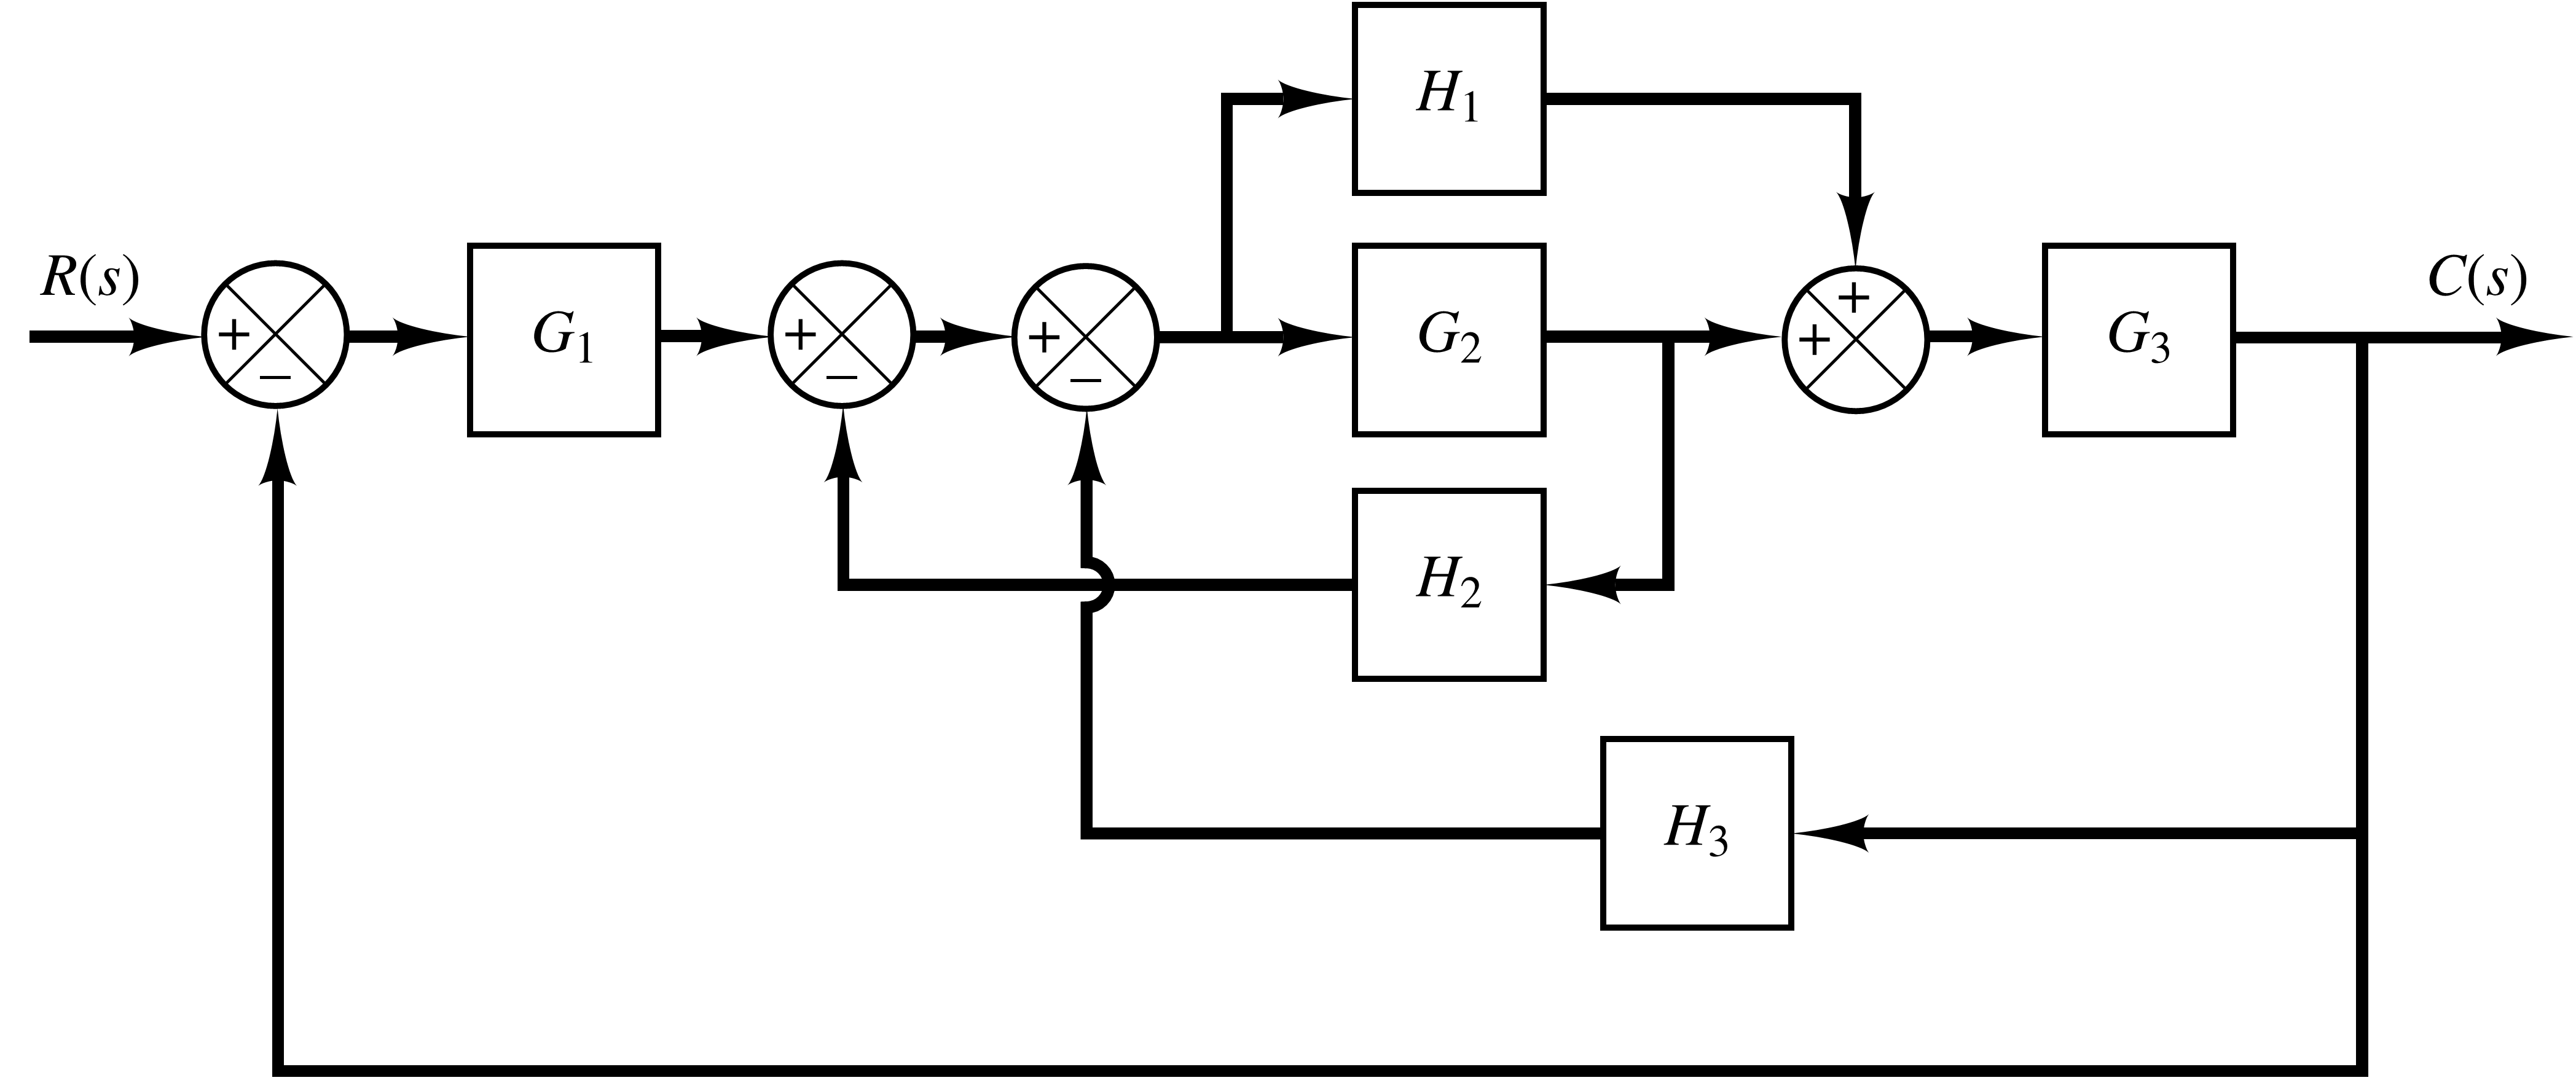
\includegraphics[width=0.8\linewidth]{Figures/Ch2/Q1}
	\caption{Block Diagram from Ogata \cite[p.60 \textbf{(B-2-3)}]{textbook:ogata}}
\end{figure}
\end{frame}

\begin{frame}
\frametitle{Another Example}
Although, the previous diagram is nice, the diagram should have thicker arrows/lines and labels need different positions, but having a diagram like this is complex enough.
\begin{figure}
	\centering
	\includegraphics[width=0.8\linewidth]{Figures/Ch2/BlockDiagramex2}
	\caption{A example from Ogata \cite[p 39, b]{textbook:ogata}}
	\label{fig:blockdiagramex2}
\end{figure}
\end{frame}
\begin{frame}[allowframebreaks]
\frametitle{Procedures for drawing a Block Diagram}
As an example, consider the RC circuit shown in Figure 2–12(a) \cite[p.38]{textbook:ogata}. The equations for
this circuit are:
\begin{align}
& i = \frac{e_i-e_o}{R} \\
& e_o = \frac{\int i dt}{C}
\end{align}
The Laplace transforms of Equations above with zero initial condition, become
\begin{align}
& I(s)=\frac{E_i(s)-E_o(s)}{R} \\
& E(s) = \frac{I(s)}{Cs}
\end{align}
Equation (2–6) represents a summing operation, and the \\
 corresponding diagram is shown in Figure 2–12(b). Equation (2–7) \\ 
 represents the block as shown in Figure 2–12(c). Assembling these two elements, we obtain the overall block diagram for the system as shown in Figure 2–12(d).
\medskip
\noindent
Block Diagram Reduction. It is important to note that blocks can be connected
in series only if the output of one block is not affected by the next following block.
\medskip
\noindent
 If there are any loading effects between the components, it is necessary to combine these
components into a single block.
\medskip
\noindent
Any number of cascaded blocks representing nonloading components can be
replaced by a single block, the transfer function of which is simply the product of the
individual transfer functions.
\medskip
\noindent
\begin{figure}
	\centering
	\includegraphics[width=0.8\linewidth]{Figures/Ch2/ex1}
	\caption{Figure 2–12 (a) RC circuit; (b) block diagram representing Equation (2–6); (c) block diagram representing Equation (2–7); (d) block diagram of the RC circuit.}
	\label{fig:chp2ex1}
\end{figure}

\end{frame}
\begin{frame}[allowframebreaks]
\frametitle{Block Diagram Reduction}
The system is said to have negative feedback if the sign at the summing junction is negative and positive
feedback if the sign is positive.
\begin{figure}
	\centering
	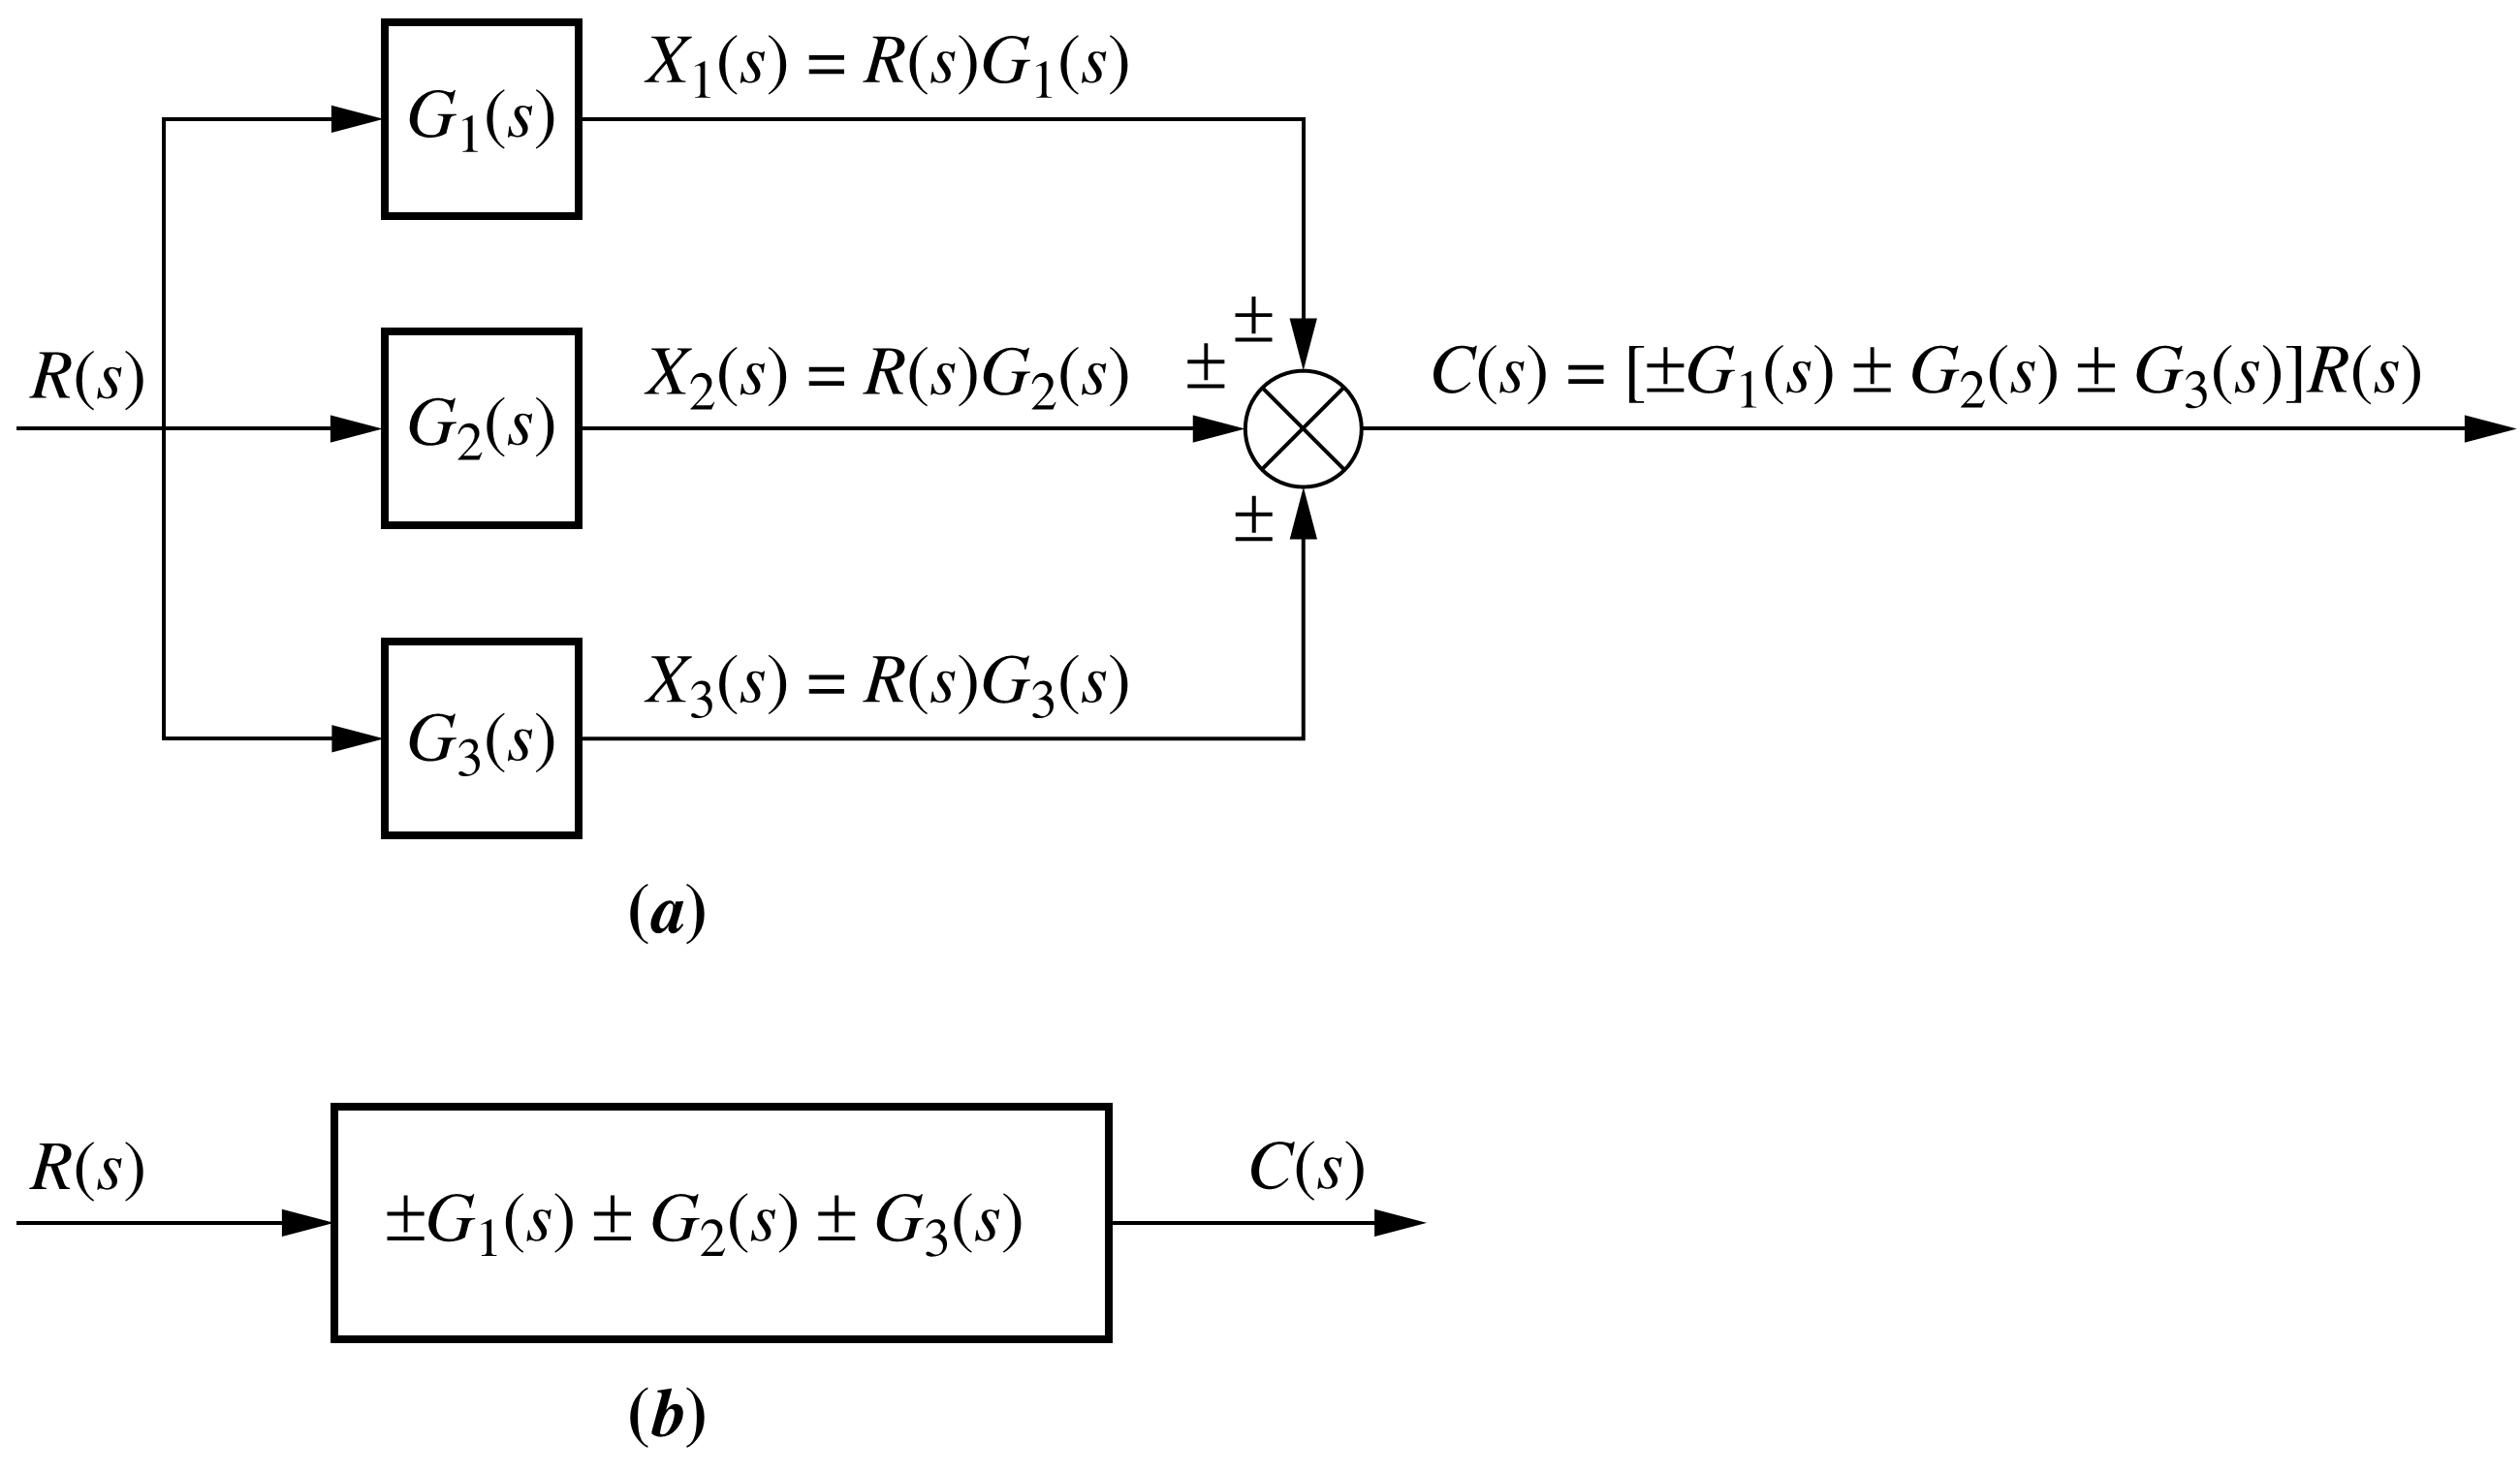
\includegraphics[width=0.7\linewidth]{Figures/Ch2/ParallelSystems}
	\caption{}
	\label{fig:parallelsystems}
\end{figure}
\begin{figure}
	\centering
	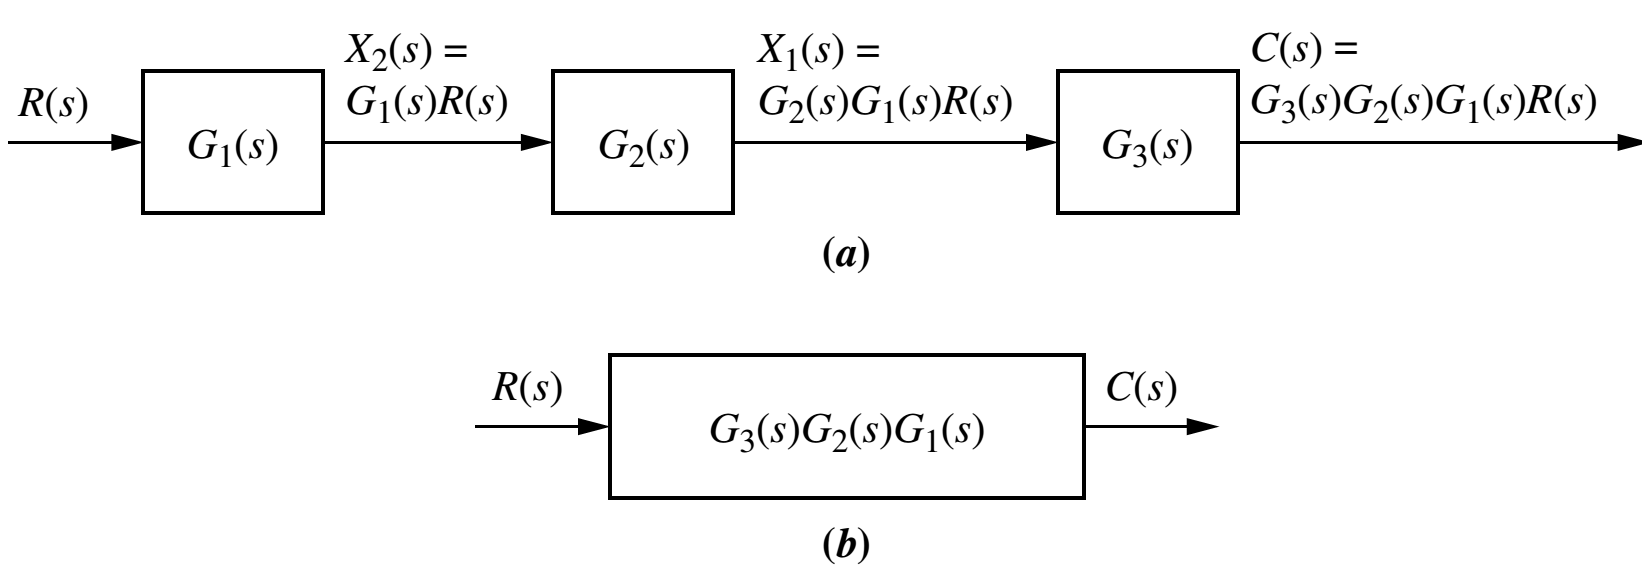
\includegraphics[width=0.7\linewidth]{Figures/Ch2/CascadingSystems}
	\caption{}
	\label{fig:cascadingsystems}
\end{figure}
\begin{figure}
	\centering
	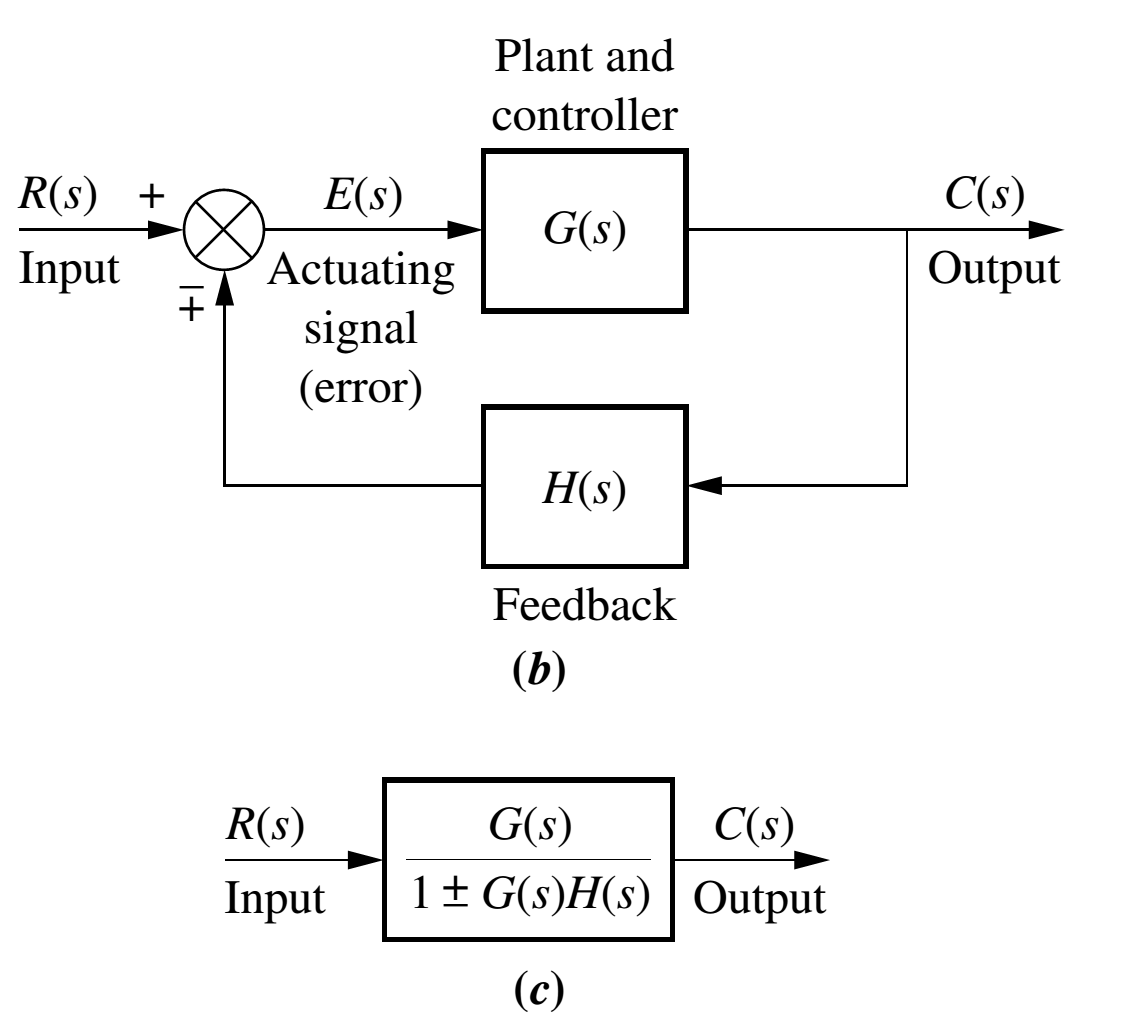
\includegraphics[width=0.5\linewidth]{Figures/Ch2/FeedbackForm}
	\caption{}
	\label{fig:feedbackform}
\end{figure}
\begin{figure}
	\centering
	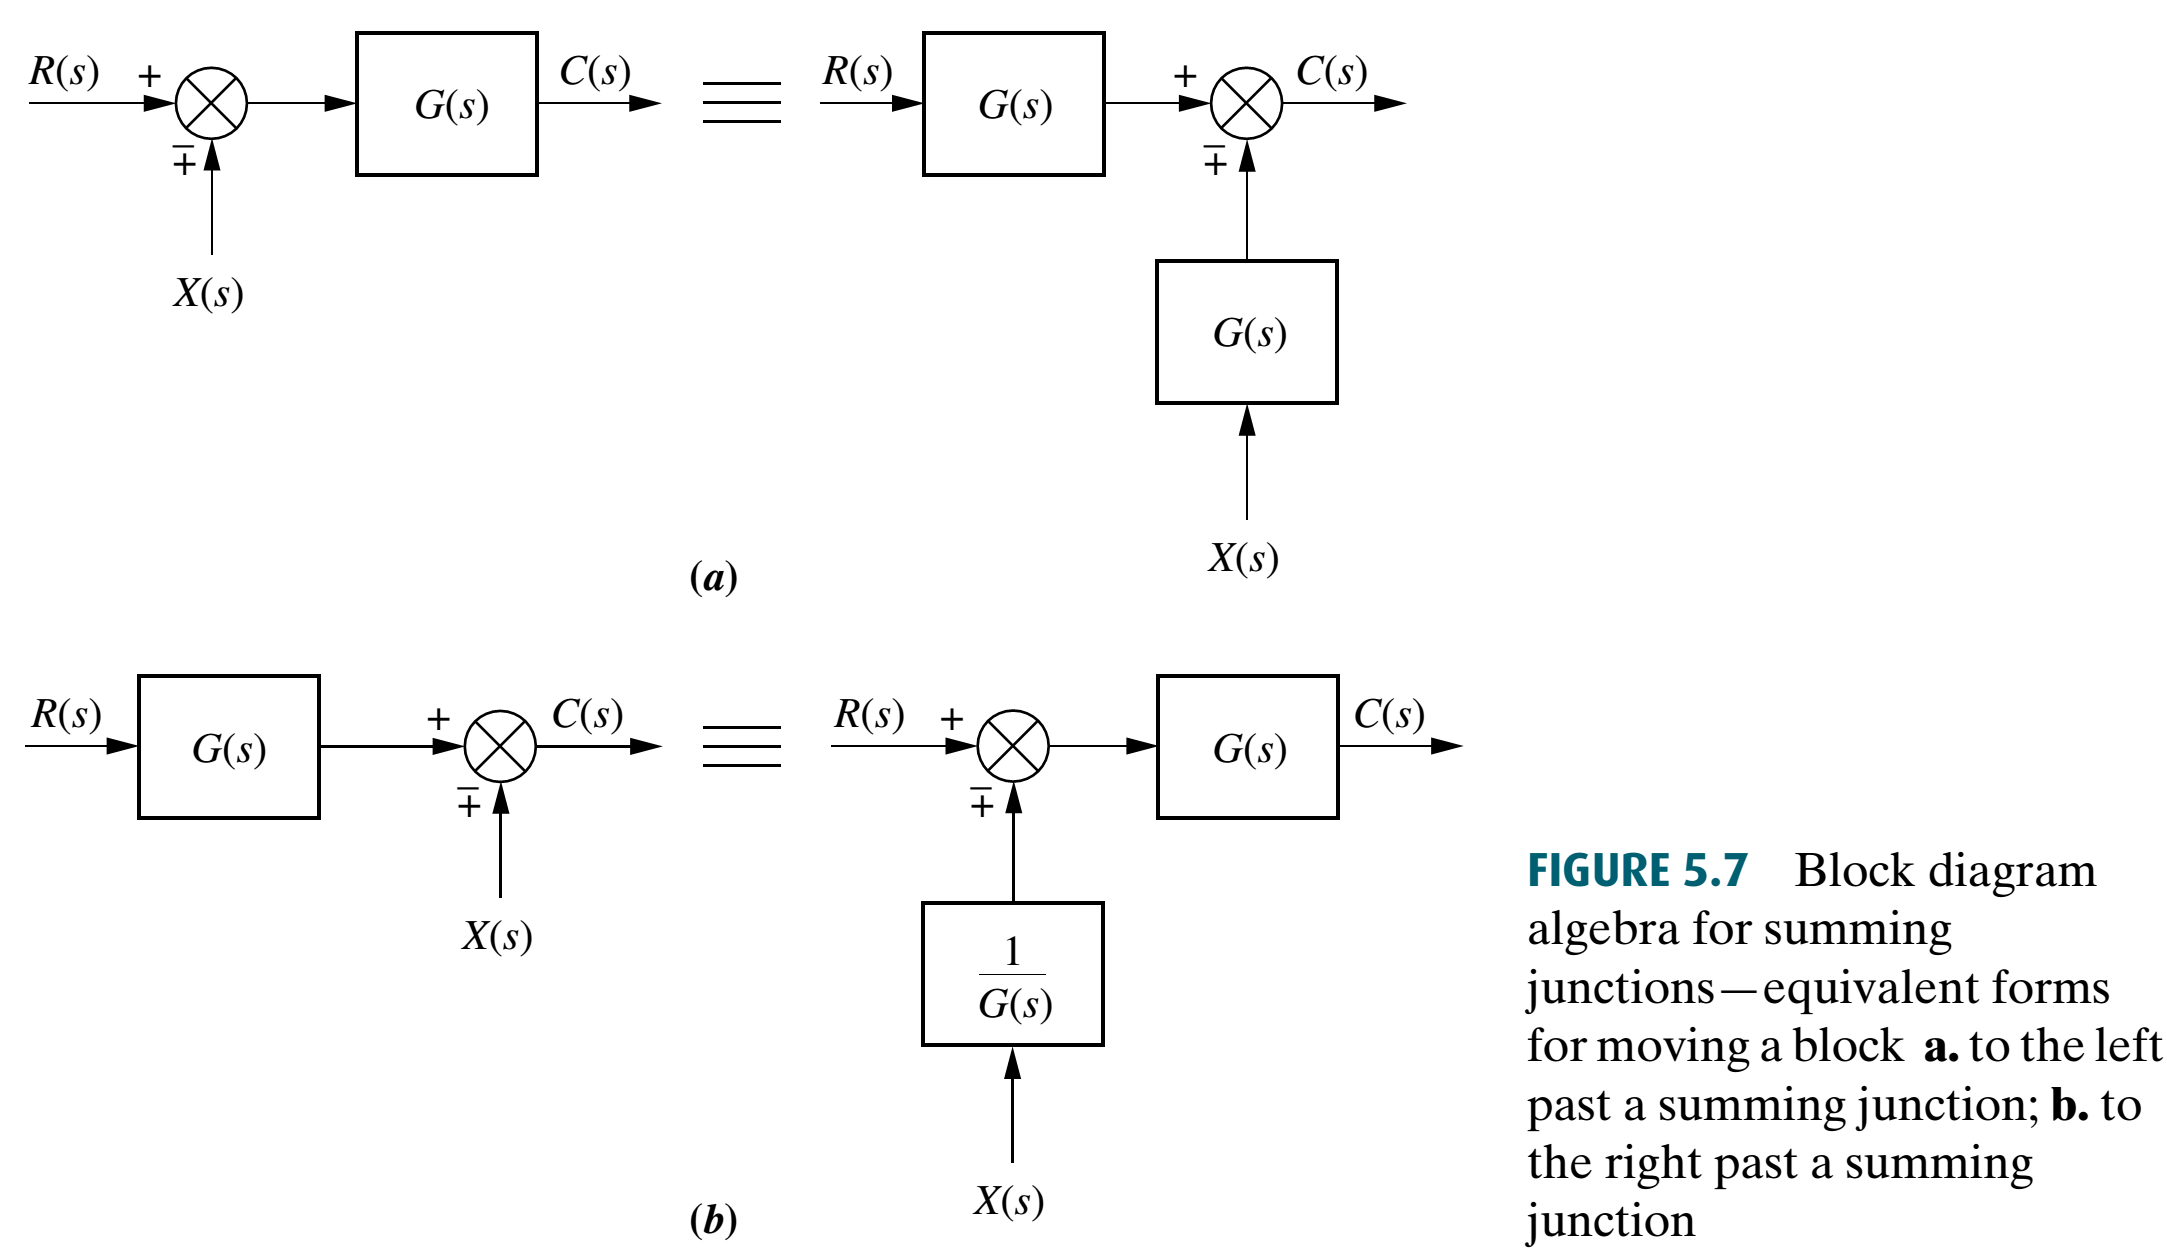
\includegraphics[width=0.7\linewidth]{Figures/Ch2/MovingBlocks1}
	\caption{}
	\label{fig:movingblocks1}
\end{figure}
\end{frame}
\begin{frame}[allowframebreaks]
\frametitle{Intro to space state analysis}

\textbf{Modern Control Theory}. The modern trend in engineering systems is toward
greater complexity, due mainly to the requirements of complex tasks and good accuracy.
\medskip
\noindent
 Complex systems may have multiple inputs and multiple outputs and may be time
varying. 
\medskip
\noindent
Because of the necessity of meeting increasingly stringent requirements on
the performance of control systems, the increase in system complexity, and easy access
to large scale computers, modern control theory, which is a new approach to the analysis and design of complex control systems, has been developed since around 1960.
\medskip
\noindent
This new approach is based on the concept of state. The concept of state by itself is not
new, since it has been in existence for a long time in the field of classical dynamics and
other fields.

\medskip
\noindent
\textbf{Modern Control Theory Versus Conventional Control Theory.}
 Modern control theory is contrasted with conventional control theory in that the former is applicable to multiple-input, multiple-output systems, which may be linear or nonlinear,
time invariant or time varying, while the latter is applicable only to \gls{LTI} single-input, single-output systems.
\medskip
\noindent
 Also, modern control theory is essentially time-domain approach and frequency domain approach (in certain cases such as
H-infinity control), while conventional control theory is a complex frequency-domain.
approach. 

\begin{align*}
x\tikzmark{x}(t)*h\tikzmark{h}(t) &= y\tikzmark{y}(t) \\[2em]
X(f) \, H(f) &= Y(f) 
\end{align*}

\begin{tikzpicture}[overlay,remember picture, > = {Circle[open,blue]}]
\draw [<->] ([yshift=-.7ex]pic cs:x) -- ++(0,-2.2em);
\draw [<->] ([yshift=-.7ex]pic cs:h) -- ++(0,-2.2em);
\draw [<->] ([yshift=-.7ex]pic cs:y) -- ++(0,-2.2em);
\end{tikzpicture}
\end{frame}

%---------------------------------------------------------
\section{Mathematical Modeling of Mechanical Systems and Electrical Systems}
\begin{frame}[allowframebreaks]
\frametitle{Chapter 3 --- Intro}
In chapter, we will model systems containing \gls{Op Amps} and \gls{DC Motors}, some knowledge of angular velocity is needed, $\Theta(s)$, refer to the other textbooks for more info.
\begin{figure}
	\centering
	\includegraphics[width=0.7\linewidth]{Figures/Ch3/ex1}
	\caption{An example Circuit with Equivalent Impedances}
	\label{fig:chp3:ex1}
\end{figure}
Finding the voltage at point A and B, $e_a$ expressed as a fraction of the input voltage, $e_i$
\begin{align*}
& e_a = \frac{iR_1}{1/C \int i d t + iR_1}e_i \\
& \frac{E_a(s)}{E_i(s)} =\frac{R_1}{1 / (Cs) + R_1} \\
& \frac{E_a(s)}{E_i(s)} =\frac{R_1Cs}{R_1Cs+1}
\end{align*}
For the voltage at point B, $e_b$
\begin{align*}
& e_b =\frac{R_3}{R_2+R_3}e_o \\
& \frac{E_b}{E_o} = \frac{R_3}{R_2+R_3}
\end{align*}
Since $E_b= E_a$, and $\displaystyle E_a(s) =\frac{R_1Cs}{R_1Cs+1}E_i(s) \quad  E_b =\frac{R_3}{R_2+R_3}E_o$ the transfer function is:
\begin{align*}
& \frac{E_o}{E_i}=\frac{R_1Cs}{R_1Cs+1}\times \frac{R_2+R_3}{R_3}= \frac{R_1R_2Cs+R_1R_3Cs}{R_1R_3Cs + R_3} = \frac{\left(1+\cfrac{R_2}{R_3}\right)s}{s+\cfrac{1}{R_1C}} \\
& \boxed{\frac{E_o}{E_1} = \frac{\left(1+\cfrac{R_2}{R_3}\right)s}{s+\cfrac{1}{R_1C}}}
\end{align*}
\end{frame}

\section{Steady State Analysis}
\begin{frame}[allowframebreaks]
\frametitle{Routh's criterion}
\begin{block}{Routh's criterion}
Routh (1874) developed a a necessary and sufficient condition for stability
based on Routh array, which states:
\end{block}
\medskip
%\begin{alertblock}{Routh's criterion}
{\bf Routh's criterion: } 
A system is stable if and only if all the elements in the first column of the
Routh array are positive.
%\end{alertbox}
\medskip

\[ \begin{array}{lllll}
\mbox{row n}   & a_0 & a_2 & a_4 & \cdots \\
\mbox{row n-1} & a_1 & a_3 & a_5 & \cdots \\
\mbox{row n-2} & b_1 & b_2 & b_3 & \cdots \\
\mbox{row n-3} & c_1 & c_2 & c_3 & \cdots \\
\cdots & \cdots & \cdots & \cdots & \cdots \\
\mbox{row 2} & * & * &  & \cdots \\
\mbox{row 1} & * &   &  & \cdots \\
\mbox{row 0} & * &   &  & \cdots \end{array} \]
{\bf Routh array: } The first two rows of the Routh array are composed of
the even and odd coefficients of the characteristic polynomial, respectively,
while the remaining rows are composed of elements derived from the first
two rows:
\medskip
The elements of the third row are computed as follows:
\medskip
\[ b_1=-\frac{det\left[\begin{array}{cc}a_0&a_2\\a_1&a_3\end{array}\right]}{a_1}
=\frac{a_1a_2-a_0a_3}{a_1} \]
\[ b_2=-\frac{det\left[\begin{array}{cc}a_0&a_4\\a_1&a_5\end{array}\right]}{a_1}
=\frac{a_1a_4-a_0a_5}{a_1} \]
\[ b_3=-\frac{det\left[\begin{array}{cc}a_0&a_6\\a_1&a_7\end{array}\right]}{a_1}
=\frac{a_1a_6-a_0a_7}{a_1} \]
The elements of the forth row are computed as follows:
\medskip
\[ c_1=-\frac{det\left[\begin{array}{cc}a_1&a_3\\b_1&b_2\end{array}\right]}{b_1}
=\frac{b_1a_3-a_1b_2}{b_1} \]
\[ c_2=-\frac{det\left[\begin{array}{cc}a_1&a_5\\b_1&b_3\end{array}\right]}{b_1}
=\frac{b_1a_5-a_1b_3}{b_1} \]
\[ c_3=-\frac{det\left[\begin{array}{cc}a_1&a_7\\b_1&b_4\end{array}\right]}{b_1}
=\frac{b_1a_7-a_1b_4}{b_1} \]
\medskip
The elements from the third row on are computed based on the determinant of a
2 by 2 array composed of the two elements of the first column of the previous
two rows and the two elements of the subsequent columns. Any missing coefficient
is represented by a zero.

%\begin{exampleblock}
{\bf Example 0: }
\[ D(s)=a_0s^3+a_1s^2+a_2s+a_3=0 \]
\[ \begin{array}{rrr}
\mbox{row 3} & a_0 & a_2 \\
\mbox{row 2} & a_1 & a_3 \\
\mbox{row 1} & (a_2a_1-a_0a_3)/a_1 & \\
\mbox{row 0} & a_3 & 
\end{array} \]
\medskip
For this system to be stable, we must have $a_2a_1-a_0a_3>0$. 
%\end{exampleblock}
%\begin{exampleblock}
As discussed previously, given the transfer function of a system:
\[
T(s)=\frac{N(s)}{D(s)}=\frac{\sum_{k=0}^m b_k s^k}{\sum_{k=0}^n a_k s^k}
=\frac{\prod_{k=1}^m (s-s_{z_k})}{\prod_{k=1}^n (s-s_{p_k})} 
\]
\medskip
(where $a_0$ is always assumed to be 1 without loss of generality), we 
can determine whether it is stable by checking if all of its poles $p_i's$
$(i=1,2,\cdots,n)$ (roots of the characteristic polynomial $D(s)$) are 
\medskip
located on the left plane (LP) of the S-plane, i.e., the real part of each
pole is negative:
\medskip
{\bf Example 1: }
\[ D(s)=s^4+2s^3+3s^2+4s+5=0 \]
\[ \begin{array}{rrrr}
\mbox{row 4}  & 1 & 3 & 5 \\
\mbox{row 3}  & 2 & 4 & 0 \\
\mbox{row 3'} & 1 & 2 & 0 \\
\mbox{row 2}  & 1 & 5 &   \\
\mbox{row 1}  & -3 &  &   \\
\mbox{row 0}  & 5  &  &   
\end{array} \]
\medskip
There are two sign changes indicating two poles on RP. Note that row 3 is divided
by 2 to become row 3' without affecting the result.
%\end{exampleblock}
\end{frame}
\begin{frame}
 \begin{itemize}
 	\item See inside Ref for details, I'll probably just end up copying and pasting questions from the assignments into this document or matlab output from my assignments, like in assignment 3.
 	\item
 \end{itemize}
\end{frame}
%---------------------------------------------------------
% Back Matter
\section{Back Matter}
\subsection{Glossaries}
\begin{frame}[allowframebreaks]
\frametitle{Glossaries}
\printglossaries
\end{frame}
%---------------------------------------------------------
\subsection{References}
\begin{frame}[allowframebreaks]%in case more than 1 slide needed
\frametitle{References}
{\footnotesize
	%\bibliographystyle{apalike}
	 \printbibliography
}
\end{frame}

%---------------------------------------------------------
\end{document}